%%
%% This is file `./samples/shortsample.tex',
%% generated with the docstrip utility.
%%
%% The original source files were:
%%
%% apa7.dtx  (with options: `shortsample')
%% ----------------------------------------------------------------------
%% 
%% apa7 - A LaTeX class for formatting documents in compliance with the
%% American Psychological Association's Publication Manual, 7th edition
%% 
%% Copyright (C) 2021 by Daniel A. Weiss <daniel.weiss.led at gmail.com>
%% 
%% This work may be distributed and/or modified under the
%% conditions of the LaTeX Project Public License (LPPL), either
%% version 1.3c of this license or (at your option) any later
%% version.  The latest version of this license is in the file:
%% 
%% http://www.latex-project.org/lppl.txt
%% 
%% Users may freely modify these files without permission, as long as the
%% copyright line and this statement are maintained intact.
%% 
%% This work is not endorsed by, affiliated with, or probably even known
%% by, the American Psychological Association.
%% 
%% ----------------------------------------------------------------------
%% 
\documentclass[jou]{apa7}

\usepackage[american]{babel}

\usepackage{csquotes}
\usepackage[style=apa,backend=biber]{biblatex}
\addbibresource{bibliography.bib}

\title{Sample APA-Style Document Using the \textsf{apa7} Package}

\authorsnames{Daniel A. Weiss}
\authorsaffiliations{Departement of Psychology, A University Somewhere}

\leftheader{Weiss}

\abstract{This demonstration paper uses the \textsf{apa7} \LaTeX\
  class to format the document in compliance with the 7th Edition of
  the American Psychological Assocation's \textit{Publication Manual.}
  The references are managed using \textsf{biblatex}.}

\keywords{APA style, demonstration}

\authornote{\addORCIDlink{Daniel A. Weiss}{0000-0000-0000-0000}, Department of Psychology, A University Somewhere

Changes of Affiliations and other info here to describe what needs to be said}

\begin{document}
\maketitle
We begin with \textcite{Shotton1989}.  We can also cite this work in
parenthesis, like this: \parencite{Lassen2006}.

Note the use of five heading levels throughout this demonstration
Method section.

\section{Method}
\subsection{Participants}
We had a lot of people in this study, show in Figure \ref{fig:Figure1}.

\begin{figure}[!htp]
    \caption{This is my figure caption.}
    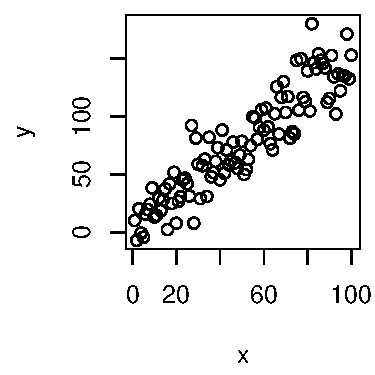
\includegraphics[bb=0in 0in 2.5in 2.5in, height=1.4in, width=1.4in]{Figure1.pdf}
    \figurenote{This is an awesome figure.}
    \label{fig:Figure1}
\end{figure}

\subsection{Materials}
Several materials were used for this project.  Some of them were
already created for prior research.

\subsubsection{Paper-and-Pencil Instrument}
We used an instrument that we found to be highly successful.

\paragraph{Reliability}
The reliability of this instrument is extraordinary.

\paragraph{Validity}
We now discuss the validity of our instrument.

\subparagraph{Face validity} The face validity is exceptionally
strong.  Everyone should be impressed.

\subparagraph{Construct validity} Also very strong.

\subsection{Design}
This section describes the study's design.

\subsection{Procedure}
The procedure was fairly straightforward, yet required
attention to detail.

\section{Results}
Table \ref{tab:ComplexTable} contains some sample data.  Our
statistical prowess in analyzing these data is unmatched.

\begin{table}[htbp]
  \vspace*{2em}
  \begin{threeparttable}
    \caption{A Complex Table}
    \label{tab:ComplexTable}
    \begin{tabular}{@{}lrrr@{}}         \toprule
    Distribution type  & \multicolumn{2}{l}{Percentage of} & Total number   \\
                       & \multicolumn{2}{l}{targets with}  & of trials per  \\
                       & \multicolumn{2}{l}{segment in}    & participant    \\ \cmidrule(r){2-3}
                                    &  Onset  &  Coda            &          \\ \midrule
    Categorical -- onset\tabfnm{a}  &    100  &     0            &  196     \\
    Probabilistic                   &     80  &    20\tabfnm{*}  &  200     \\
    Categorical -- coda\tabfnm{b}   &      0  &   100\tabfnm{*}  &  196     \\ \midrule
    \end{tabular}
    \tablenote{All data are approximate.

            \tabfnt{a}Categorical may be onset.
            \tabfnt{b}Categorical may also be coda.

            \tabfnt{*}\textit{p} < .05.
            \tabfnt{**}\textit{p} < .01.
         }
  \end{threeparttable}
\end{table}

\section{Discussion}
This is a lengthy and erudite discussion.  It demonstrates amazing
skill in interpreting the results for the masses.

\printbibliography

\end{document}

%% 
%% Copyright (C) 2021 by Daniel A. Weiss <daniel.weiss.led at gmail.com>
%% 
%% This work may be distributed and/or modified under the
%% conditions of the LaTeX Project Public License (LPPL), either
%% version 1.3c of this license or (at your option) any later
%% version.  The latest version of this license is in the file:
%% 
%% http://www.latex-project.org/lppl.txt
%% 
%% Users may freely modify these files without permission, as long as the
%% copyright line and this statement are maintained intact.
%% 
%% This work is not endorsed by, affiliated with, or probably even known
%% by, the American Psychological Association.
%% 
%% This work is "maintained" (as per LPPL maintenance status) by
%% Daniel A. Weiss.
%% 
%% This work consists of the file  apa7.dtx
%% and the derived files           apa7.ins,
%%                                 apa7.cls,
%%                                 apa7.pdf,
%%                                 README,
%%                                 APA7american.txt,
%%                                 APA7british.txt,
%%                                 APA7dutch.txt,
%%                                 APA7english.txt,
%%                                 APA7french.txt,
%%                                 APA7german.txt,
%%                                 APA7ngerman.txt,
%%                                 APA7greek.txt,
%%                                 APA7czech.txt,
%%                                 APA7turkish.txt,
%%                                 APA7spanish.txt,
%%                                 APA7endfloat.cfg,
%%                                 Figure1.pdf,
%%                                 shortsample.tex,
%%                                 longsample.tex, and
%%                                 bibliography.bib.
%% 
%%
%% End of file `./samples/shortsample.tex'.
